\documentclass[12pt, letterpaper]{article}
\usepackage[spanish]{babel}
\usepackage[utf8]{inputenc}
\usepackage{amsmath}
\usepackage{amssymb}
\usepackage{graphicx}
\usepackage{geometry}
\usepackage{fancyhdr}
\usepackage{enumitem}
\usepackage{cmbright}
\usepackage[T1]{fontenc}

\geometry{letterpaper, margin=2.5cm, headheight=33pt}

\pagestyle{fancy}
\fancyhf{}
\fancyhead[L]{
\includegraphics[height=1cm]{Logouagrm.png}}
\fancyhead[R]{
\includegraphics[height=1cm]{Logocont.png}}
\fancyfoot[C]{\thepage}

\begin{document}

% CARÁTULA
\begin{titlepage}
    \centering
    
\includegraphics[height=3.5cm]{Logouagrm.png}\hfill
    
\includegraphics[height=3.5cm]{Logocont.png}
    \vspace{1cm}
    
    \textbf{\Large UNIVERSIDAD AUTÓNOMA GABRIEL RENÉ MORENO} \\
    \vspace{0.3cm}
    \textbf{\large FACULTAD DE CIENCIAS CONTABLES} \\
    \vspace{0.3cm}
    \textbf{\large CARRERA DE CONTADURÍA PÚBLICA} \\
    \vspace{2cm}
    
    \textbf{\LARGE ESTADÍSTICA II} \\
    \vspace{0.3cm}
    \textbf{\large MAT-260 GRUPO EP} \\
    \vspace{2cm}
    
    \textbf{\Large PRÁCTICO N° 1} \\
    \vspace{0.3cm}
    \textbf{\Large ANÁLISIS COMBINATORIO} \\
    \vspace{2cm}
    
    \textbf{\large DOCENTE:} \\
    \textbf{MSc. Anselmo Salguero Arano} \\
    \vspace{1cm}
    
    \textbf{\large FECHA:} \\
    \textbf{abril de 2026} \\
    \vfill
    \textbf{Santa Cruz de la Sierra - Bolivia}
\end{titlepage}

\newpage

% ==================== LEY DE ADICIÓN ====================
\section*{Ley de Adición}

\begin{center}
    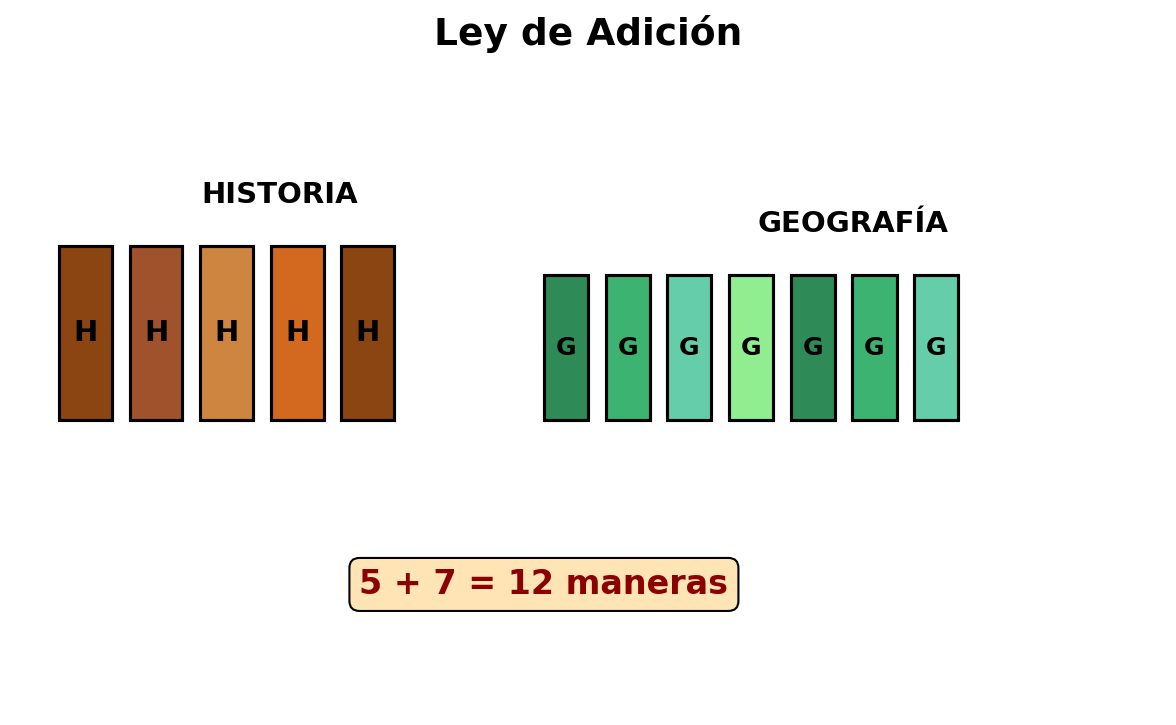
\includegraphics[width=0.7\textwidth]{ley_adicion_libros.png}
\end{center}

\begin{enumerate}[label=\arabic*.]
    \item En una biblioteca hay 5 libros de historia y 7 de geografía. ¿De cuántas maneras se puede seleccionar un libro?
\end{enumerate}

\vspace{0.5cm}

% ==================== LEY DE MULTIPLICACIÓN ====================
\section*{Ley de Multiplicación}

\begin{center}
    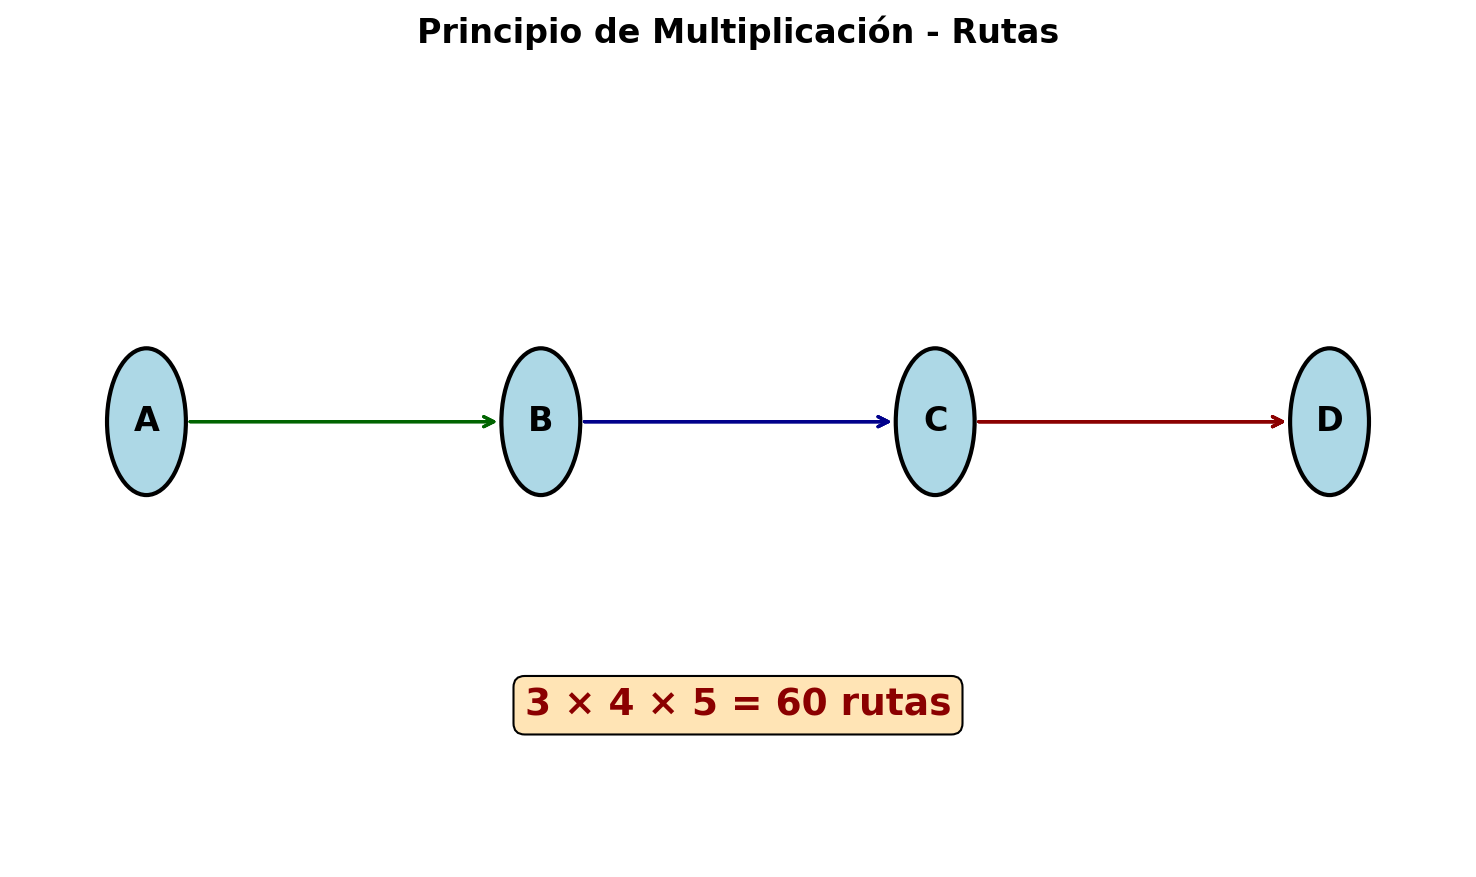
\includegraphics[width=0.7\textwidth]{principio_multiplicacion_rutas.png}
\end{center}

\begin{enumerate}[label=\arabic*.]
    \setcounter{enumi}{1}
    \item ¿Cuántas rutas existen para ir desde el punto A al punto D pasando por B y C, si hay 3 caminos de A a B, 4 de B a C y 5 de C a D?
    \item Un código de acceso consta de 2 letras (A-Z, 26 letras) seguidas de 3 dígitos (0-9). ¿Cuántos códigos diferentes se pueden formar si se permite la repetición?
    \item Un restaurante ofrece un menú con 4 entradas, 6 platos principales y 5 postres. ¿Cuántas comidas diferentes de 3 platos (entrada, principal y postre) se pueden pedir? ¿Y si el plato principal puede ser elegido dos veces?
    \item En una carrera participan 12 corredores. ¿De cuántas formas pueden ocuparse los 3 primeros lugares (oro, plata y bronce)?
\end{enumerate}

\vspace{0.5cm}

% ==================== PERMUTACIONES ====================
\section*{Permutaciones}

\begin{enumerate}[label=\arabic*.]
    \setcounter{enumi}{5}
    \item Cierto comité de economistas consta de siete integrantes, en este comité se premia la puntualidad de sus asistentes dado que se hace uso de una mesa (No circular) con 5 sillas quedando dos de los integrantes de pie los cuales son los últimos en llegar.
    
    \begin{center}
        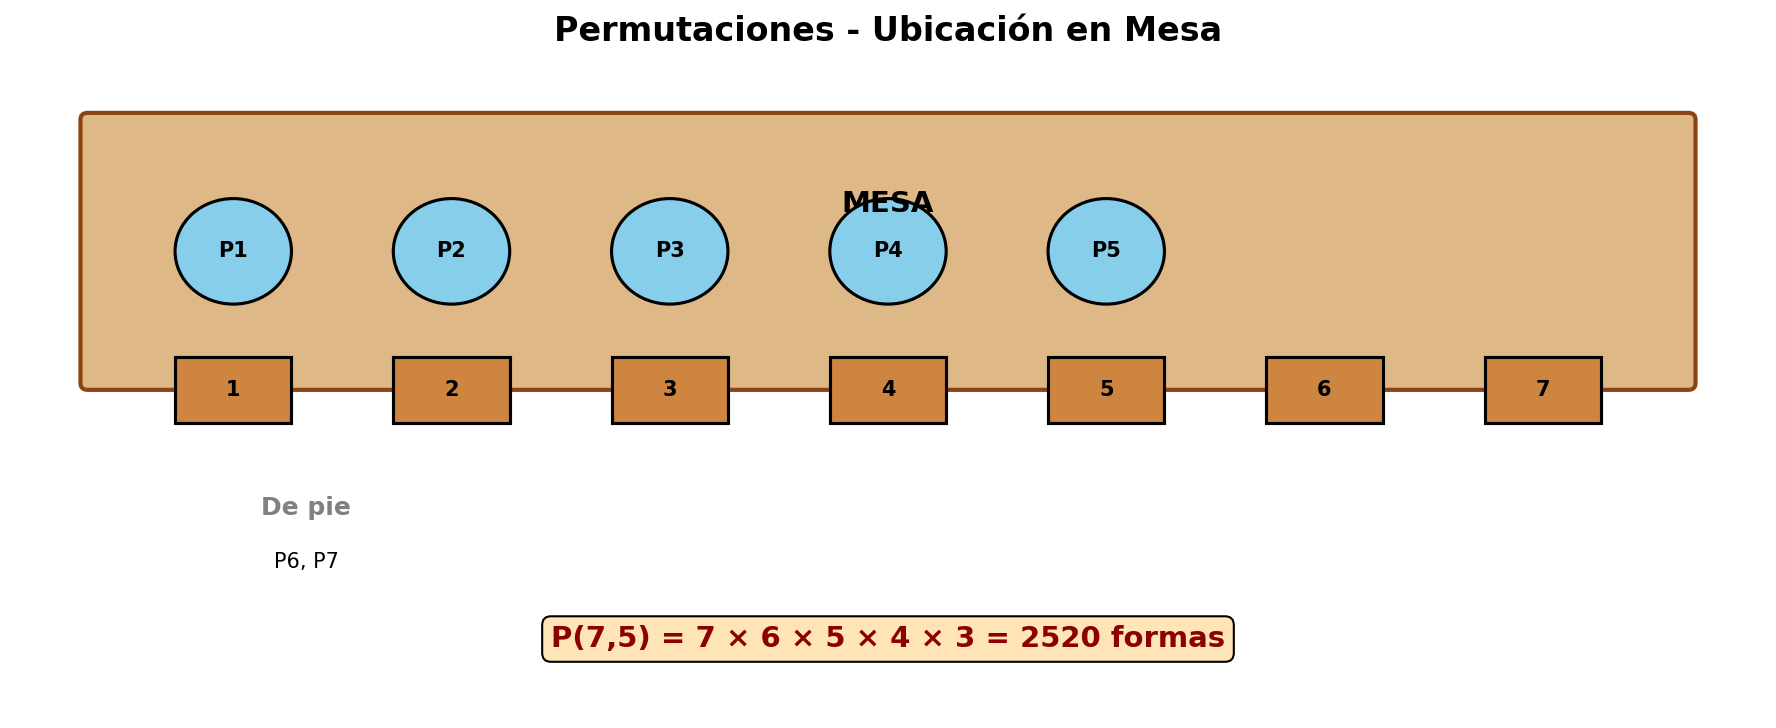
\includegraphics[width=0.6\textwidth]{permutaciones_mesa.png}
    \end{center}
    
    \begin{enumerate}[label=\alph*)]
        \item ¿De cuántas formas posibles pueden ubicarse los economistas en la mesa del comité?
        \item De los 7 integrantes 4 son hombres y 3 son mujeres. ¿De cuántas formas posibles pueden ubicarse los economistas si se debe alternar hombre - mujer y las mujeres deben ir en los lugares pares?
        
        \begin{center}
            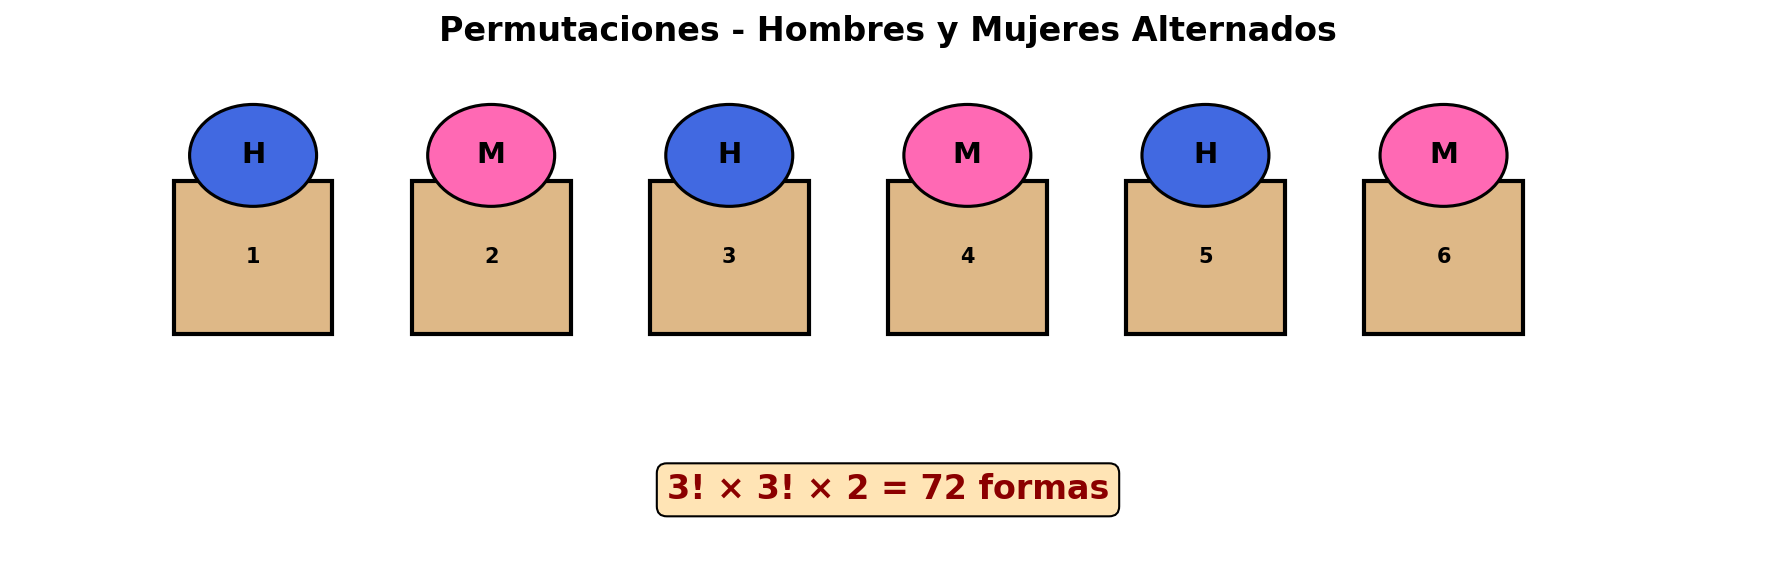
\includegraphics[width=0.6\textwidth]{permutaciones_alternadas.png}
        \end{center}
    \end{enumerate}
    
    \item Se desea ordenar en una fila de asiento a 5 personas, de los cuales 2 son varones, 2 mujeres y 1 niño, en cada acomodo que se realice el niño deberá permanecer entre las 2 mujeres.
    
    \item Un tren de pasajeros comprende 3 coches para equipaje, dos coches de primera clase y tres de segunda clase. ¿De cuántas formas se puede arreglar los coches, si los vagones de equipaje deben ir adelante y los 3 de segunda clase al final?
    
    \item ¿De cuántas maneras distribuiríamos 3 billetes de Bs. 50 y 4 billetes de Bs. 100 en una misma línea?
    
    \item ¿Cuántas permutaciones se pueden hacer con las letras de la palabra COOPERADORES, si se considera que las O deben estar juntas?
    
    \item ¿Cuántos números de 4 cifras diferentes se pueden formar con los dígitos 1, 2, 3, 4, 5, 6, si el número debe ser mayor que 4000?
    
    \item Un grupo de 6 amigos (3 hombres y 3 mujeres) van al cine. ¿De cuántas formas pueden sentarse en una fila de 6 asientos si los hombres y las mujeres deben alternarse?
    
    \item ¿Cuántas palabras diferentes (con o sin sentido) se pueden formar con las letras de la palabra "MATEMATICAS"? Considere las repeticiones de letras.
    
    \begin{center}
        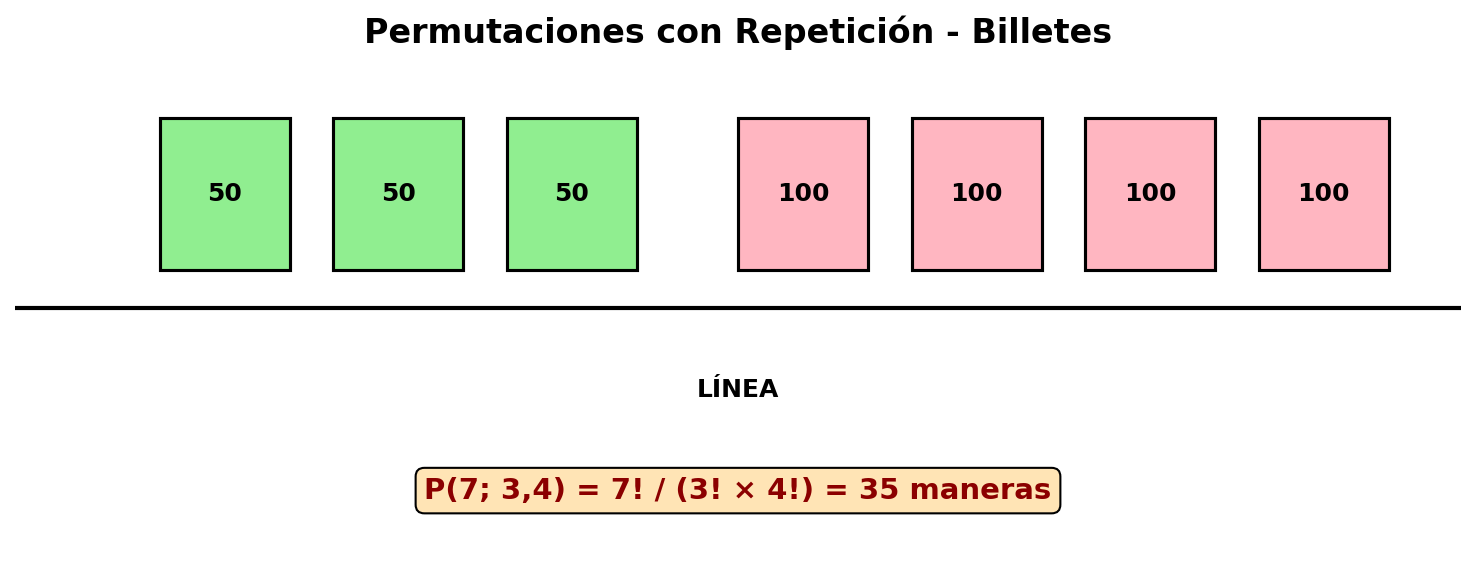
\includegraphics[width=0.6\textwidth]{permutaciones_repeticion.png}
    \end{center}
    
    \item ¿Cuántas señales diferentes se pueden formar con 8 banderas de colores distintos si se izan exactamente 4 banderas en un mástil y el orden sí importa?
    
    \item Una persona tiene 10 libros diferentes y quiere colocarlos en un estante. ¿De cuántas formas puede ordenarlos si 3 libros específicos deben estar siempre juntos?
    
    \item Una compañía tiene 8 candidatos para ocupar 4 puestos distintos en una nueva oficina. ¿De cuántas formas pueden asignarse los puestos si 2 de los candidatos son hermanos y no pueden ocupar puestos juntos?
\end{enumerate}

\newpage

% ==================== COMBINATORIA ====================
\section*{Combinatoria}


\begin{enumerate}[label=\arabic*.]
    \setcounter{enumi}{18}
    \item ¿Cuántos grupos de 6 letras (combinaciones) se pueden formar con las letras de la palabra AMIGAS , tomando en cuenta que el orden no es importante?
    
    \item ¿Cuántas señales diferentes se pueden formar con 10 banderas distintas, levantando al menos 3 y no más de 6 banderas?
    
    \item ¿De cuántas formas pueden escogerse 4 personas de 5 parejas de casados si la selección debe ser de dos hombres y dos mujeres?
    
    \item A partir de un grupo de 12 personas, de las cuales 8 son varones y 4 son mujeres.
     
    \begin{enumerate}[label=\alph*)]
        \item Para formar un comité de 4 personas con una mujer y 3 varones, ¿de cuántas maneras?
        \item Si el comité está conformado por 4 mujeres y 8 varones, ¿de cuántas maneras?
    \end{enumerate}
    
    \item ¿Cuántos comités diferentes pueden seleccionarse entre 7 hombres y 4 mujeres si deben constituirse de:
    \begin{enumerate}[label=\alph*)]
        \item 3 hombres y 2 mujeres
        \item Un comité de 5 personas con al menos cuatro hombres.
    \end{enumerate}
    \begin{center}
        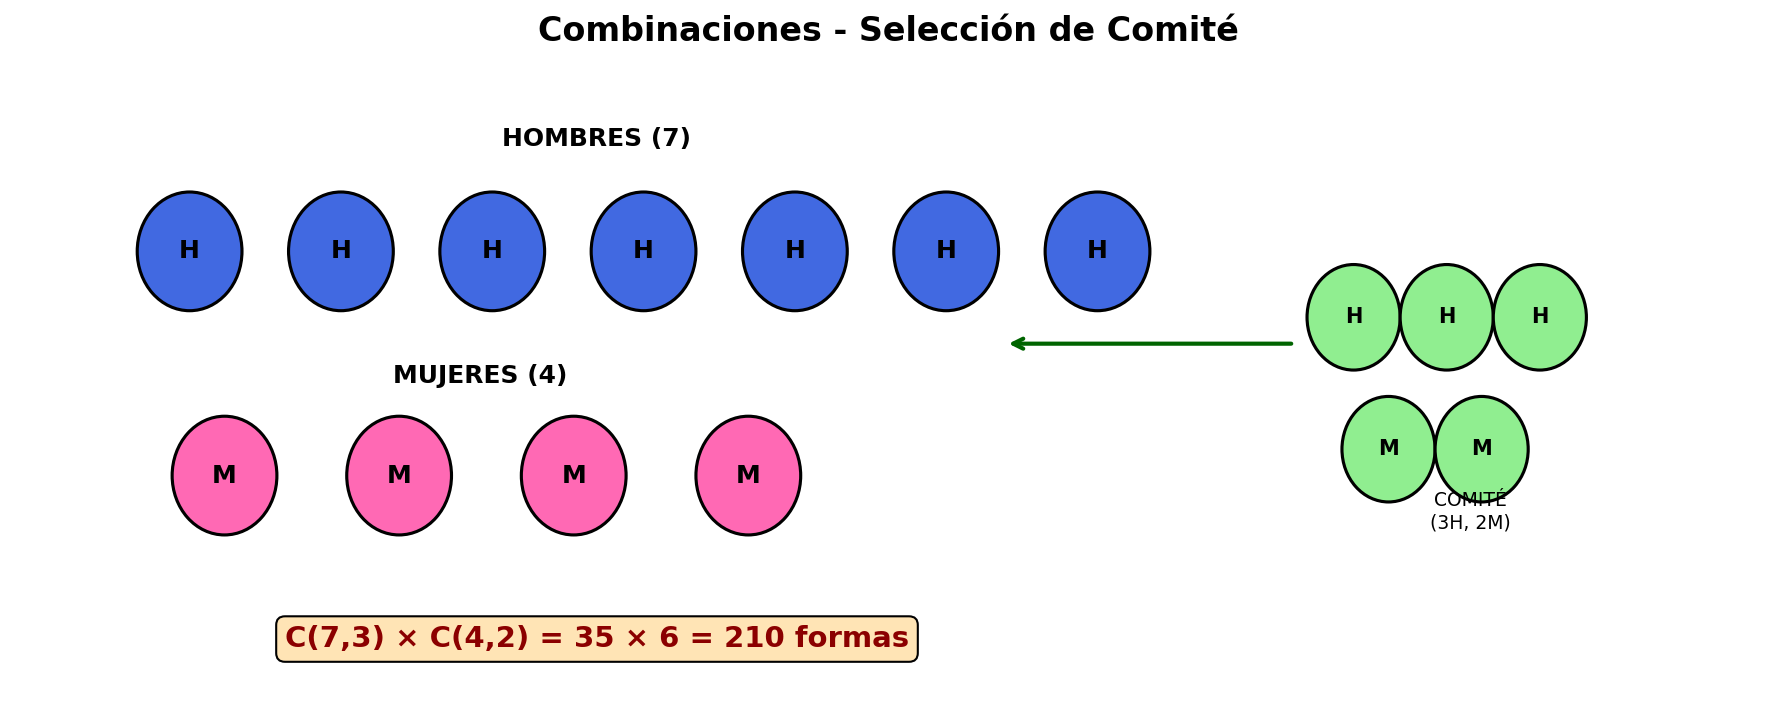
\includegraphics[width=0.6\textwidth]{combinaciones_comite.png}
    \end{center}
\end{enumerate}

\begin{enumerate}[label=\arabic*.]
    \setcounter{enumi}{23}
    \item Un estudiante debe responder 8 de 10 preguntas en un examen.
    \begin{enumerate}[label=\alph*)]
        \item ¿De cuántas formas puede hacerlo?
        \item ¿Y si debe responder al menos 3 de las primeras 5?
    \end{enumerate}
    
    \item Un estudiante debe elegir 4 preguntas de un total de 7. ¿De cuántas formas si las primeras 2 son obligatorias?
    
    \item Un taller tiene 8 máquinas, 3 averiadas. Se seleccionan 4. ¿Cuántas formas si al menos 2 están averiadas?
    
    \item En una caja hay 5 bolas rojas, 4 azules y 3 verdes. ¿De cuántas formas se pueden extraer 4 bolas todas del mismo color?
    
    \begin{center}
        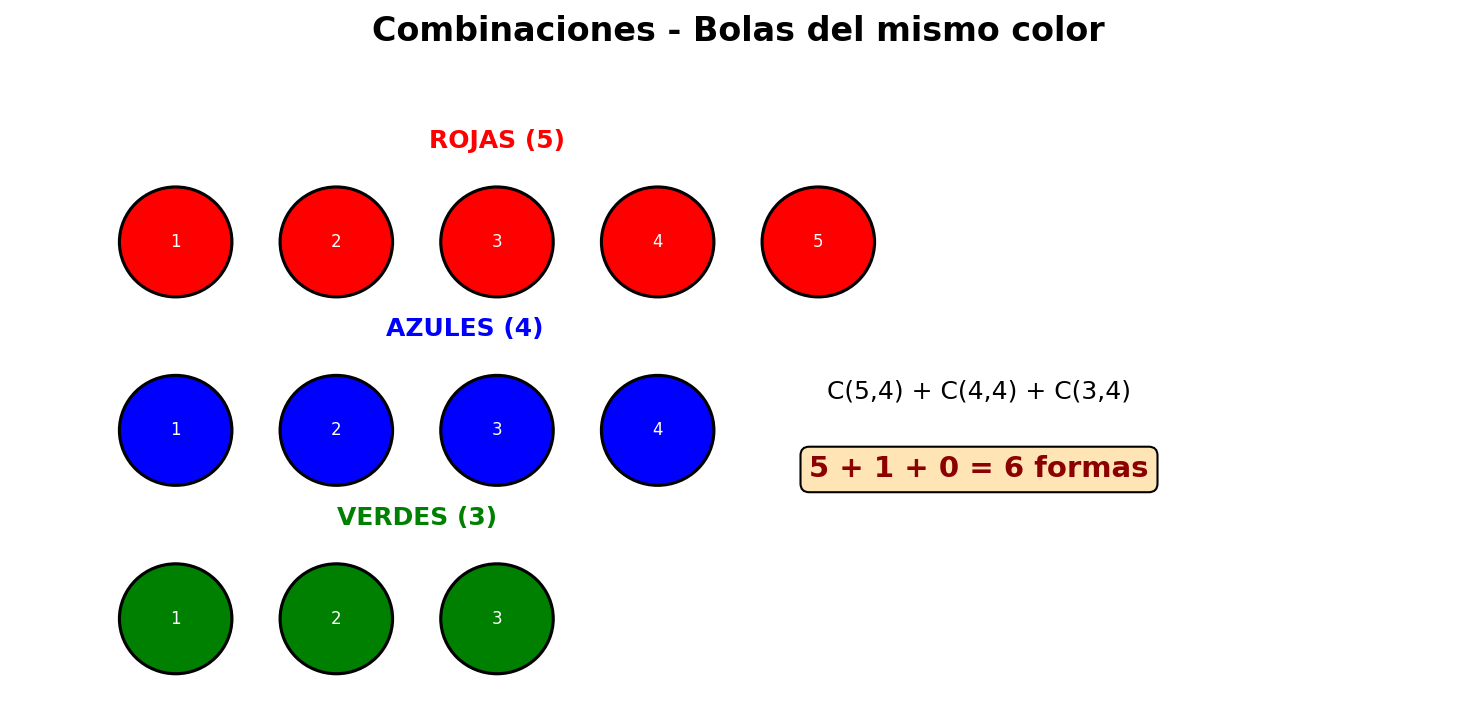
\includegraphics[width=0.6\textwidth]{combinaciones_bolas.png}
    \end{center}
    
    \item Un profesor tiene 12 preguntas: 5 álgebra, 4 geometría, 3 trigonometría. ¿De cuántas formas puede seleccionar 6 con al menos 2 de cada tema?
    
    \item En una fiesta hay 12 personas. ¿Cuántos apretones de manos diferentes si cada persona saluda una vez a cada otra?
    
    \begin{center}
        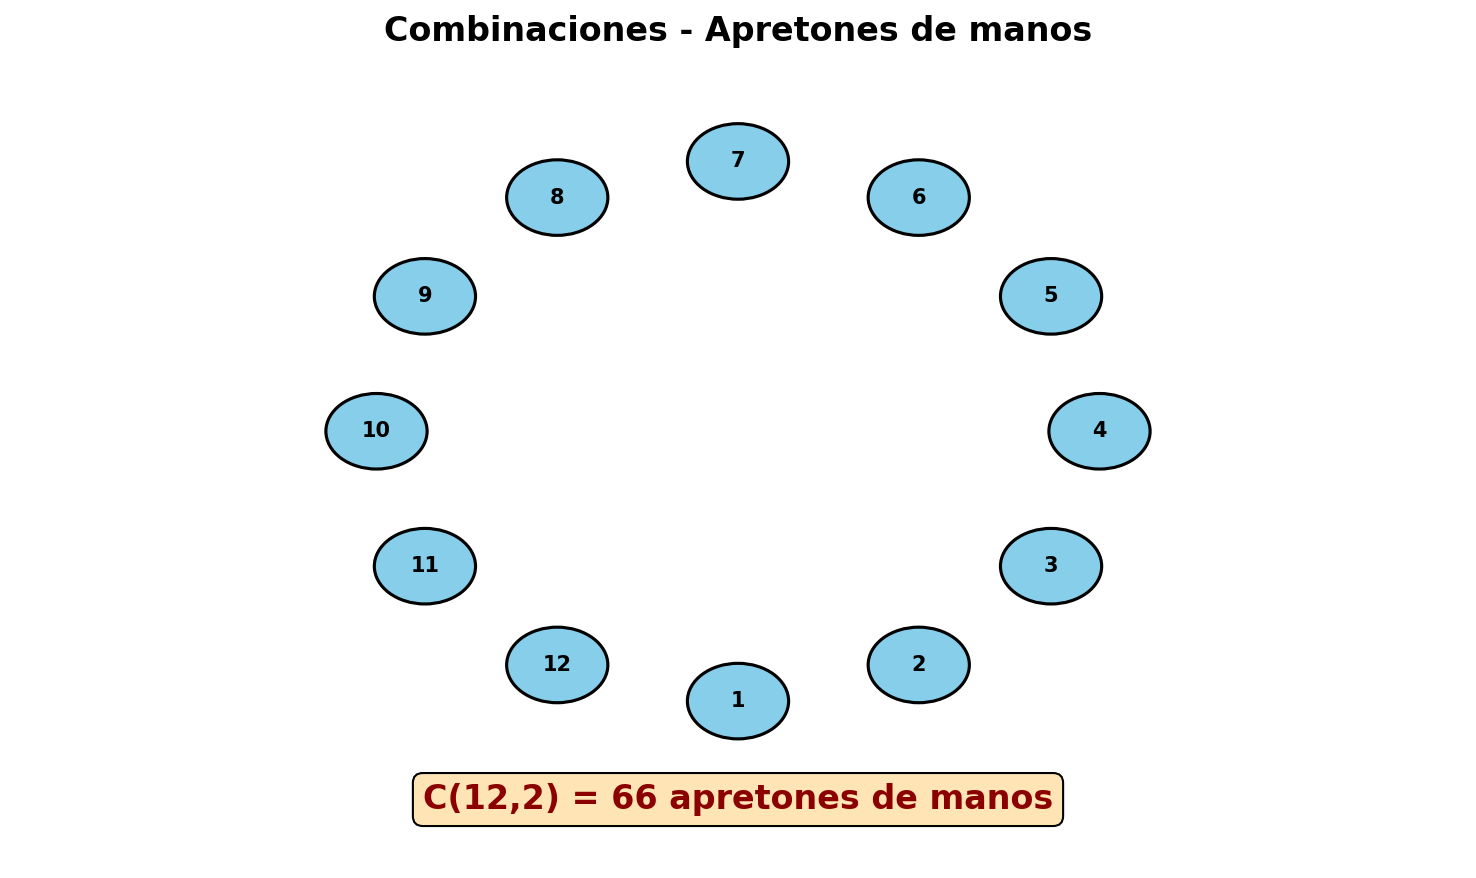
\includegraphics[width=0.6\textwidth]{combinaciones_apretones.png}
    \end{center}
    
    \item ¿De cuántas formas pueden acomodarse 7 personas en un auto de 5 espacios, si solo 3 saben conducir y quedan 2 fuera, importando el orden?
    
    \item En una reunión hay 6 matemáticos y 5 físicos. ¿De cuántas formas formar un comité de 5 con al menos un matemático y un físico?
 
\end{enumerate}
   \begin{center}
    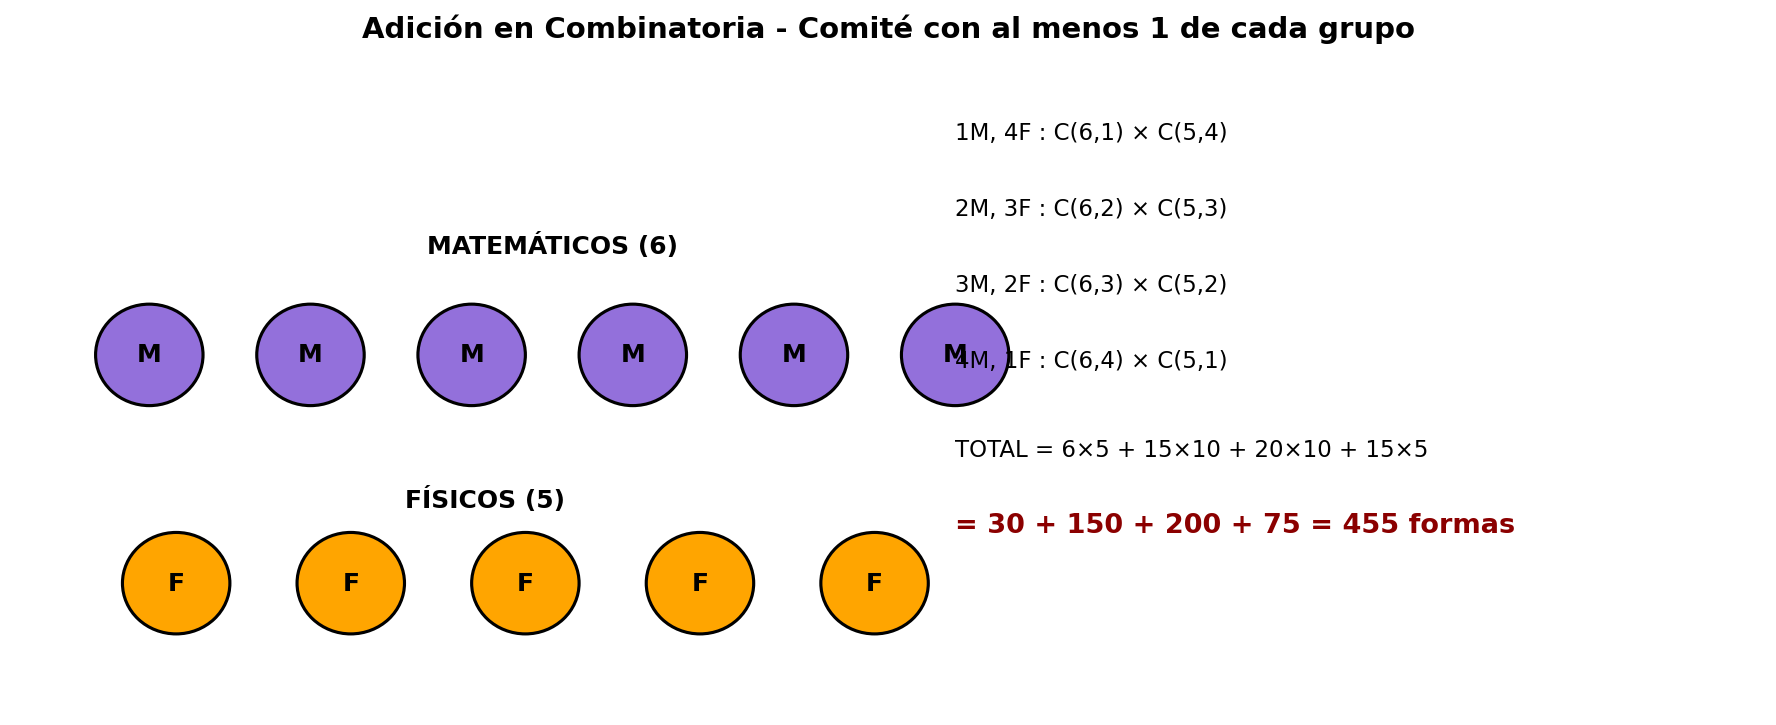
\includegraphics[width=0.7\textwidth]{combinaciones_adicionales.png}
    \end{center}

\end{document}